\chapter{\chatextlogicalRepresentation}\label{cha:logicalRepresentation}

Propositional logics describes systems with $\atomorder$ boolean variables, which are called atoms and denoted by $\atomicformulaof{\atomenumerator}$ for $\atomenumeratorin$.
Indices $\catindexof{\atomenumerator}\in[2]$ to the atoms $\atomenumeratorin$ enumerate the $2^\atomorder$ states of these systems, which are called worlds.
In each world indexed by $\shortcatindices=\catindices$ the indices $\atomicformulaof{\atomenumerator}$ encode whether the corresponding variable is $\truesymbol$. 

% Propositional logics
The epistemological commitments of propositional logics are whether the state is $\truesymbol$ or $\falsesymbol$ reflected by the coordinate of the one-hot encoding being $1$ or $0$.
Intuitively this describes, whether a specific world can be the state of a factored system.
Propositional logic amounts to reason about boolean variables, which are categorical variables with $2$ possible values.
Such boolean tensors have already appeared as base measures in the representation of probability distributions in \charef{cha:probRepresentation}.

Before discussing the semantics and syntax of propositional formulas, we first investigate how Boolean can be represented by vectors in order to mechanize their processing based on contractions.



\sect{Encoding of Booleans}\label{sec:booleanEncoding}

Booleans are variables valued by $\truthset$ and consist a basic data structure.

\subsect{Representation by coordinates}

To represent Booleans by categorical variables $\catvariable$ with two states we use the index interpretation function
\begin{align*}
	\indexinterpretation:[2]\rightarrow\truthset%\rightarrow\ozset
\end{align*}
defined as
\begin{align*}
	\indexinterpretationat{1} = \truesymbol%} = 1
	\quad \text{and} \quad \indexinterpretationat{0} = \falsesymbol \, .
\end{align*}

% Outlook: General interpretation maps
In \defref{def:subsetEncoding} in \parref{par:three} will define encodings of arbitrary sets based on index interpretation maps.

% Group homomorphism
One motivation for this particular choice of the interpretation function $\indexinterpretation$ is the effective execution of the conjunction as we show in the next Lemma.

\begin{lemma}
	$\indexinterpretation$ is a homomorphism between the groups
	\begin{align*}
		\big(\ozset,\cdot\big)  \quad \text{and} \quad \big(\truthset,\land\big) \, .
	\end{align*}
\end{lemma}
\begin{proof}
	It suffices to notice, that for arbitrary $\truthstateof{0},\truthstateof{1}\in\ozset$ we have
	\begin{align*}
		\indexinterpretationat{\truthstateof{0} \cdot \truthstateof{1}}
		= \indexinterpretationat{\truthstateof{0}} \land \indexinterpretationat{\truthstateof{1}}  \, .
	\end{align*}
\end{proof}
	
% Interpretation of boolean contraction and type conversion application
Based on this homomorphism, contractions of boolean tensors, in which all variables are kept open, can be regarded as parallel calculations of the conjunction $\land$ encoded by $\indexinterpretation$.
This homomorphism is further applied in type conversion in dynamically-typed languages (e.g. in $\mathrm{python}$ \cite{python_software_foundation_python_2025}).

% Nonlinearity issues
Operations like the negation fail to be linear and are only affine linear, since for $\truthstate\in\truthset$ we have
\begin{align}\label{eq:affineLinearNegation}
 	\invindexinterpretationat{\lnot\truthstate} = 1 - \invindexinterpretationat{\truthstate}  \, .
\end{align}
Since any logical connective can be represented as a composition of conjunctions and negations, any logical connective corresponds with an affine linear function on the interpreted truth values.
Direct applications of this insight to execute logical calculus will be discussed later in \secref{sec:effectiveCalculus}.
For our purposes here, we would like to execute logical connective based on single contractions and avoid summations over them.
This is why we call the negation representation as in \eqref{eq:affineLinearNegation} the affine representation problem, which we in the following want to resolve.

% Disjunction central interpretation
While in this work, we will always encode boolean states by $\indexinterpretation$, other index interpretation functions could be chosen.
For example, the interpretation
	\[ \indexinterpretationof{\lor}:\ozset\rightarrow\truthset \]
defined as
    	\[ \indexinterpretationofat{\lor}{0} = \truesymbol \quad \text{and} \quad \indexinterpretationofat{\lor}{1} = \falsesymbol \, , \]
results is a homomorphism between the groups	
	\[ \big(\ozset,\cdot\big) \quad \text{and} \quad \big(\truthset,\lor\big)  \, . \]
While placing the disjunction $\lor$ as the logical connective effectively executed by contractions, the negation will for arbitrary interpretations mapping onto $\ozset$ remain the function %\eqref{eq:affineLinearNegation}
\begin{align*}
 	\invindexinterpretationofat{\lor}{\lnot\truthstate} = 1 - \invindexinterpretationofat{\lor}{\truthstate}  \, .
\end{align*}
Thus, the problem of affine linear operations cannot be resolved by a clever choice of an interpretation function with image in $\ozset$. 


\subsect{Representation by basis vectors} % This is what Basis Calculus does! Refer to that here?

While contractions can just perform conjunctions, we need a representation trick to extend the contraction expressivity to arbitrary connectives and resolve the affine representation problem.
To this end we now compose $\indexinterpretation$ with the one-hot encoding $\onehotmap$ and get an encoding
\begin{align*}
	\onehotmap\circ\invindexinterpretation : \truthset \rightarrow \ozbasisset \, ,
\end{align*}
where $\catvariable$ is a categorical variable with $\catdim=2$.
For any $\truthstate\in\truthset$ we have
\begin{align*}
	\onehotmap\circ\invindexinterpretationat{\truthstate} =
	\begin{bmatrix}
		\invindexinterpretationat{\lnot\truthstate} \\
		\invindexinterpretationat{\truthstate}
	\end{bmatrix}  \, .
\end{align*}


% Resolving the affine representation problem
Performing the negation now amounts to switching the coordinates of the encoded vector, which can be performed by contraction with a transposition matrix
\begin{align*}
	\rencodingofat{\lnot}{\headvariableof{\lnot},\catvariable} = 
	\begin{bmatrix}
		0 & 1 \\
		1 & 0
	\end{bmatrix} \, ,
\end{align*}
where in this notation we always understand the first variable $\catvariable$ as the row index selector and the second variable $\headvariableof{\notucon}$ as the column index selector.
We then have
\begin{align*}
	\onehotmap\circ\invindexinterpretationat{\lnot\truthstate}[\headvariableof{\lnot}]
	= \contractionof{\rencodingofat{\notucon}{\headvariableof{\notucon},\catvariable},\onehotmap\circ\invindexinterpretationat{\truthstate}[\catvariable]}{\headvariableof{\notucon}} \, .
\end{align*}
We therefore arrived at our aim to resolve the affine representation problem and have found a procedure to represent logical negations by a contraction, which is a linear operation.
Besides negations, we will show in this chapter, that arbitrary logical formulas can be represented by contractions.

\subsect{Coordinate and Basis Calculus}

Our findings on the encoding of booleans hint towards more general schemes to encode information into boolean tensors, which will be explored in more detail in \charef{cha:coordinateCalculus} and \charef{cha:basisCalculus}.
When each coordinate in a boolean tensor represents one in $\ozset$ interpreted boolean we call the scheme coordinate calculus.
In basis calculus on the other hand, booleans are represented by elements of $\ozbasisset$.
In that scheme, there are pairs of two coordinates (building slice vectors of the tensors), which are restricted to be different from each other.
This amounts to posing a global directionality constraint on the boolean tensor, as will be shown in \theref{the:rencodingDirected}.

\sect{Semantics of Propositional Formulas}

% Structure
We now choose a semantic centric approach to propositional logic, by defining formulas as boolean tensors.
Then we investigate the corresponding syntax of formulas as specification of a tensor network decomposition of the relational encoding of formulas.

\subsect{Formulas}

% Intro of formulas
Logics is especially useful in interpreting boolean tensors representing Propositional Knowledge Bases, based on connections with abstract human thinking.
To make this more precise, we associate each such tensor is associated with a formula $\exformula$ being a composition of the atomic variables with logical connectives as we proof next.

\begin{definition}\label{def:formulas}
	A propositional formula $\formulaat{\shortcatvariables}$ depending on $\atomorder$ atoms $\catvariableof{\atomenumerator}$ is a boolean-valued tensor
	\begin{align*}
		\formulaat{\shortcatvariables} : \atomstates \rightarrow \ozset \subset \rr \, .
	\end{align*}
	We call a state $\shortcatindices \in \atomstates$ a model of a propositional formula $\formula$, if
	\begin{align*}
		\formulaat{\indexedshortcatvariables}=1 \, .
	\end{align*}
	If there is a model to a propositional formula, we say the formula is satisfiable.
\end{definition}

% Boolean Tensors
The propositional formulas coincide therefore with the boolean tensors (see \defref{def:booleanTensor}).


% Decomposition into model sums
Since propositional formulas are binary valued tensors, the generic decomposition of \lemref{lem:tensorBasisDecomposition} simplifies to
\begin{align}\label{eq:formulaModelDecomposition}
	\formulaat{\shortcatvariables} = \sum_{\catindices\in\atomstates} \formulaat{\indexedcatvariables} \cdot \onehotmapofat{\shortcatindices}{\shortcatvariables} \\
	= \sum_{\catindices\in\atomstates \, : \, \formulaat{\indexedcatvariables}=1}  \onehotmapofat{\catindices}{\shortcatvariables} \, .
\end{align}
Thus, any propositional formula is the sum over the one-hot encodings of its models.
This is equal to the encoding of the set of models, which will be introduced in \charef{cha:basisCalculus} (see \defref{def:subsetEncoding}).

We depict this decomposition in the diagrammatic notation by
\begin{center}
	\begin{tikzpicture}[scale=0.35, thick] % , baseline = -3.5pt

%\draw[->-] (2,-1)--(2,1) node[midway,right] {\tiny $\catvariableof{\exformula}$};
\draw (-1,-1) rectangle (5,-3);
\node[anchor=center] (text) at (2,-2) {\small ${\exformula}$};
\draw[] (0,-3)--(0,-5) node[midway,left] {\tiny $\randomxof{0}$}; 
\draw[] (1.5,-3)--(1.5,-5) node[midway,left] {\tiny $\randomxof{1}$}; 
\node[anchor=center] (text) at (3,-4) {$\cdots$};
\draw[] (4,-3)--(4,-5) node[midway,right] {\tiny $\randomxof{\atomorder\shortminus1}$}; 


\node[anchor=center] (text) at (7,-2) {${=}$};

\node[anchor=center] (text) at (12,-2.5) {${\sum\limits_{\atomindices\in\atomstates}}$};
\node[anchor=center] (text) at (12,-4) {\tiny $\exformula(\atomindices)=1$};

\begin{scope}[shift={(19.5,1)}]

%\draw (-2,1) rectangle (4,-1);
%\node[anchor=center] (text) at (1,0) {\small $\onehotmapof{\exformula(\atomindices)}$};
%\draw[->-] (1,1)--(1,3) node[midway,right] {\tiny $\catvariableof{\exformula}$};

\draw (-3,-2) rectangle (-1,-4);
\node[anchor=center] (text) at (-2,-3) {\small $\onehotmapof{\atomlegindexof{0}}$};
\draw[->-] (-2,-4)--(-2,-6) node[midway,right] {\tiny $\catvariableof{0}$};

\node[anchor=center] (text) at (1,-3) {\small $\cdots$};

\draw (3,-2) rectangle (5,-4);
\node[anchor=center] (text) at (4,-3) {\small $\onehotmapof{\atomlegindexof{\atomorder\shortminus1}}$};
\draw[->-] (4,-4)--(4,-6) node[midway,right] {\tiny $\catvariableof{\atomorder\shortminus1}$};

\end{scope}

\end{tikzpicture}
\end{center}




% Maps to multiple formulas -> Later?
%We can extend the map to factored systems of multiple formulas, by using \defref{def:formulas} as coordinate maps.
%This is exactly what we will study by Bayesian Propositional Networks.
%We will make use of redundancies in the maps to get an efficient representation based on decompositions.





%% Semantic approach
We here chose a semantic approach to propositional logic in contrary to the standard syntactical approach.
Instead of defining formulas by connectives acting on atomic formulas, we define them here as binary valued functions of the states of a factored system.
They are interpreted by marking possible states as models, given the knowledge of $\exformula$.
The syntactical side will then be introduced later by studying decompositions of formulas.


%\begin{figure}[h]
%\begin{center}
%	\begin{tikzpicture}[scale=0.35, thick] % , baseline = -3.5pt

%\draw[->-] (2,-1)--(2,1) node[midway,right] {\tiny $\catvariableof{\exformula}$};
\draw (-1,-1) rectangle (5,-3);
\node[anchor=center] (text) at (2,-2) {\small ${\exformula}$};
\draw[] (0,-3)--(0,-5) node[midway,left] {\tiny $\randomxof{0}$}; 
\draw[] (1.5,-3)--(1.5,-5) node[midway,left] {\tiny $\randomxof{1}$}; 
\node[anchor=center] (text) at (3,-4) {$\cdots$};
\draw[] (4,-3)--(4,-5) node[midway,right] {\tiny $\randomxof{\atomorder\shortminus1}$}; 


\node[anchor=center] (text) at (7,-2) {${=}$};

\node[anchor=center] (text) at (12,-2.5) {${\sum\limits_{\atomindices\in\atomstates}}$};
\node[anchor=center] (text) at (12,-4) {\tiny $\exformula(\atomindices)=1$};

\begin{scope}[shift={(19.5,1)}]

%\draw (-2,1) rectangle (4,-1);
%\node[anchor=center] (text) at (1,0) {\small $\onehotmapof{\exformula(\atomindices)}$};
%\draw[->-] (1,1)--(1,3) node[midway,right] {\tiny $\catvariableof{\exformula}$};

\draw (-3,-2) rectangle (-1,-4);
\node[anchor=center] (text) at (-2,-3) {\small $\onehotmapof{\atomlegindexof{0}}$};
\draw[->-] (-2,-4)--(-2,-6) node[midway,right] {\tiny $\catvariableof{0}$};

\node[anchor=center] (text) at (1,-3) {\small $\cdots$};

\draw (3,-2) rectangle (5,-4);
\node[anchor=center] (text) at (4,-3) {\small $\onehotmapof{\atomlegindexof{\atomorder\shortminus1}}$};
\draw[->-] (4,-4)--(4,-6) node[midway,right] {\tiny $\catvariableof{\atomorder\shortminus1}$};

\end{scope}

\end{tikzpicture}
%\end{center}
%\caption{Direct interpretation of a propositional formula $\exformula$ as a tensor.
%	The tensor is the sum of the one hot encodings of its models.
%	While the one hot encodings are directed, their sum is not.}
%\label{fig:formulaDirect} 
%\end{figure}

%% Intro of connectives
%Logical connectives are basic building blocks of such formulas and can be understood by simple computations represented in truth tables.
% Here truth tables?
%We call each combination of atomic formulas with connectives a formula.

\subsect{Relational encoding of formulas}


%% Direct and Relational interpretation of $\exformula$
There are two ways to represent formulas by tensors.
One way is to understand $[2]$ as subset of $\rr$ and interpreting the formula directly as a tensor (as in \defref{def:formulas}).
Another way is to understand $[2]$ as the possible values of a categorical variable.
% Maps between factored systems
Following this second perspective, formulas are maps between factored systems, where the image system is the factored systems of atoms and the target system the atomic system defined by a variable $\formulavar$ representing the formula satisfaction.
%Following this perspective, formulas are maps between the factored systems of atoms and the atomic system of the formula.
We can then build the relational encoding (\defref{def:functionRepresentation}) of that map to represent the formula (see Figure~\ref{fig:formulaRencoding}).

%\begin{definition}[Relation Encoding of Formulas] % Own definition, since a reinterpretation of the formula
Given a factored system with $\atomorder$ atoms $\shortcatvariables$ and a propositional formula $\formula$, the relational encoding of $\formula$ (see \defref{def:functionRepresentation}) is the tensor
\begin{align*}
	\rencodingofat{\formula}{\formulavar,\shortcatvariables} \in  \left(\atomspace \right) \otimes \rr^2
\end{align*}
decomposable as
\begin{align} 
	\rencodingofat{\formula}{\formulavar,\shortcatvariables} 
	= & \sum_{\shortcatindices\in\atomstates}  \onehotmapofat{\shortcatindices}{\shortcatvariables} \otimes \onehotmapofat{\formulaat{\indexedshortcatvariables}}{\formulavar} \, . 
\end{align}
%\end{definition}

%% More general relational encodings
We can build relational encodings more generally of any tensors, where we identify the image of the tensor with the states of a categorical variable.
Exactly for propositional formulas, this construction will lead to Boolean image variables.


\begin{lemma}\label{lem:formulaEncodingDecomposition}
	For any formula $\formula$ we have
	\begin{align*}
		\rencodingofat{\formula}{\formulavar,\shortcatvariables}
		= \formulaat{\shortcatvariables} \otimes \tbasisat{\formulavar}
		+ \lnot\formulaat{\shortcatvariables} \otimes  \fbasisat{\formulavar} \, .
	\end{align*}
	In particular
	\begin{align*}
		 \formulaat{\shortcatvariables} = \contractionof{
		\rencodingofat{\formula}{\formulavar,\shortcatvariables},\tbasisat{\formulavar}
		}{\shortcatvariables} \, .
	\end{align*}
\end{lemma}
\begin{proof}
%% Decomposition
	We can decompose relational encodings of formulas into the sum (see Figure~\ref{fig:formulaRencoding}) % ! Not a tensor network decomposition !
	\begin{align} 
		 \rencodingofat{\formula}{\formulavar,\shortcatvariables}  
		 = & \fbasisat{\formulavar} \otimes \left( \sum_{\formulazerocoordinates}  \onehotmapofat{\shortcatindices}{\shortcatvariables} \right) \\
		 + & \tbasisat{\formulavar} \otimes \left( \sum_{\formulaonecoordinates}  \onehotmapofat{\shortcatindices}{\shortcatvariables} \right)
	\end{align}
	where the second term sums up the models of $\formula$ and the first one the models of $\lnot\formula$.
\end{proof}


% Comparison with direct interpretation
Compared with the direct interpretation of a formula as a tensor and the decomposition into models in Equation~\ref{eq:formulaModelDecomposition}, we notice that the relational encoding also represents encoding of worlds where the formula is not satisfied.
This representation is required to represent arbitrary propositional formulas by contracted tensor networks of its components, as will be investigated in the following sections.

%% Coordinatewise 
The relational encoding $\rencodingof{\exformula}$ has slices
\begin{align*}
	\contractionof{\rencodingof{\exformula},\onehotmapof{\shortcatindices}}{\formulavar} 
		\rencodingofat{\exformula}{\indexedshortcatvariables,\formulavar}
	= \begin{cases}
		\tbasis[\formulavar] & \text{if the world $\shortcatindices$ is a model of $\exformula$}  \\
		\fbasis[\formulavar] & \text{else}\, .
		\end{cases}
\end{align*}
The contractions of the relational encoding therefore calculate whether an assignment of atoms is a model of the formula, using basis calculus (see \theref{the:basisCalculus}).

\begin{figure}[h]
\begin{center}
	\input{./PartI/tikz_pics/logic_representation/formula_rencoding.tex}
\end{center}
\caption{Relational encoding of a propositional formula. 
The encoding is a sum of the one hot encodings of all states of the factored system in a tensor product with basis vectors, which encode whether the state is a model of the formula.
The tensor is directed, since any contraction with an encoded state results in the basis vector evaluating the formula, which we called basis calculus.
}
\label{fig:formulaRencoding} 
\end{figure}


\sect{Syntax of Propositional Formulas}

Relational encodings of propositional formulas are especially useful when representing function compositions by the representation of their components (see \theref{the:compositionByContraction}).
In propositional logics, the syntax of defining propositional formulas is oriented on compositions of formulas by connectives. % Quantifications will be studied in the FOL Chapter.
We in this section investigate the decomposition schemes of relational encodings into tensor networks of component encodings for binary tensors following propositional logic syntax.

\subsect{Atomic Formulas}

We call atomic formulas the most granular formulas, which are not splitted into compositions of other formulas.
Our syntactic decomposition of propositional formulas will then investigate, how any propositional formula can be represented by these.

\begin{definition}
	The tensors $\formulaofat{\atomenumerator}{\shortcatvariables}$ defined for $\shortcatindices\in\atomstates$ as
	\begin{align*}
		\formulaofat{\atomenumerator}{\indexedshortcatvariables}
		= \catindexof{\atomenumerator}
	\end{align*}
	are called atomic formulas.
\end{definition}

Atomic formulas and their relational encodings have an especially compelling representation.

\begin{theorem}
	Any atomic formula $\formulaofat{\atomenumerator}{\shortcatvariables}$ is represented as
	\begin{align*}
		\formulaofat{\atomenumerator}{\indexedshortcatvariables}
		= \contractionof{\tbasisat{\catvariableof{\atomenumerator}}}{\shortcatvariables}
		= \tbasisat{\catvariableof{\atomenumerator}} \otimes \onesat{\catvariableof{[\catorder]/\{\atomenumerator\}}}  \, .
	\end{align*}

	The relational encoding of any atomic formula $\atomicformulaofat{\atomenumerator}{\shortcatvariables}$ has a tensor decomposition by
	\begin{align*}
		\rencodingofat{\atomicformulaof{\atomenumerator}}{\headvariableof{\atomorder},\shortcatvariables}
		= \contractionof{\identityat{\catvariableof{\atomenumerator},\headvariableof{\atomenumerator}}}{\shortcatvariables}
		= \identityat{\catvariableof{\atomenumerator},\headvariableof{\atomenumerator}} \otimes \onesat{\catvariableof{[\catorder]/\{\atomenumerator\}}} \, .
	\end{align*}
	The decomposition is depicted in a network diagram as
	\begin{center}
		\begin{tikzpicture}[scale=0.35,thick] % , baseline = -3.5pt

\drawatomcore{3.5}{-8}{$\bencodingof{\formulaof{\atomenumerator}}$}
\drawatomindices{3.5}{-12}	
\draw[->-] (5.5,-9)--(5.5,-7) node[midway,right] {\tiny $\headvariableof{\atomenumerator}$};

\node[anchor=center] (text) at (10,-10) {${=}$};

\draw (12,-9) rectangle (15,-11); 
\node[anchor=center] (text) at (13.5,-10) {\small $\ones$}; 
\draw[-<-] (12.5,-11)--(12.5,-13) node[midway,left] {\tiny $\catvariableof{0}$};
\node[anchor=center] (text) at  (13.5,-12) {$\cdots$};
\draw[-<-] (14.5,-11)--(14.5,-13) node[midway,right] {\tiny $\catvariableof{\atomenumerator\shortminus1}$};

\node[anchor=center] (text) at (16.25,-10) {\small $\otimes$}; 

\draw[->-] (18.5,-9)--(18.5,-7) node[midway,right] {\tiny $\headvariableof{\atomenumerator}$};
\draw (17.5,-9) rectangle (19.5,-11);
\node[anchor=center] (text) at (18.5,-10) {\small $\delta$}; 
\draw[-<-]  (18.5,-11)--(18.5,-13) node[midway,right] {\tiny $\catvariableof{\atomenumerator}$};

\node[anchor=center] (text) at (20.75,-10) {\small $\otimes$}; 

\begin{scope}[shift={(10,0)}]

\draw (12,-9) rectangle (15,-11); 
\node[anchor=center] (text) at (13.5,-10) {\small $\ones$}; 
\draw[-<-]  (12.5,-11)--(12.5,-13) node[midway,left] {\tiny $\catvariableof{\atomenumerator+1}$};
\node[anchor=center] (text) at  (13.5,-12) {$\cdots$};
\draw[-<-]  (14.5,-11)--(14.5,-13) node[midway,right] {\tiny $\catvariableof{\atomorder\shortminus1}$};

\node[anchor=center] (text) at  (16.5,-13) {$.$};

\end{scope}

\end{tikzpicture}
	\end{center}
\end{theorem}
\begin{proof}
	We have by definition
	\begin{align*}
		\rencodingofat{\atomicformulaof{\atomenumerator}}{\headvariableof{\atomenumerator},\shortcatvariables}
		=& \sum_{\catindices\in\atomstates} \onehotmapofat{\catindices}{\shortcatvariables} \otimes \onehotmapofat{\formulaofat{\atomenumerator}{\indexedcatvariables}}{\headvariableof{\atomenumerator}} \\
		=& \left( \onehotmapofat{0,0}{\catvariableof{\atomenumerator},\headvariableof{\atomenumerator}} +
		\onehotmapofat{1,1}{\catvariableof{\atomenumerator},\headvariableof{\atomenumerator}} \right) \otimes \onesat{\catvariableof{\secatomenumerator}\, : \, \secatomenumerator \neq \atomenumerator} \\
		=& \contractionof{\identityat{\catvariableof{\atomenumerator},\headvariableof{\atomenumerator}}}{\shortcatvariables,\headvariableof{\atomenumerator}} \, .
	\end{align*} 
\end{proof}

\subsect{Syntactical combination of formulas}

Propositional formulas are elements of tensor spaces with $\atomorder$ axis. 
The number of coordinates thus grows exponentially with the number of atoms, which is
\begin{align*}
	\dimof{\atomspace} = 2^{\atomorder} \, .
\end{align*}
When the number of atoms is large, the naive representation of formula tensors will be thus intractable.
In contrast, typcial logical formulas appearing in practical knowledge bases are sparse in the sense that they have short representations in a logical syntax.
Motivated by this consideration we now discuss propositional syntax and investigate the sparse decomposition of formula tensors along their formula structure to avoid the curse of dimensionality.

%% Propositional Syntax
In logical syntax formulas are described by atomic formulas recursively connected via connectives. 
We show, that representations of logical connectives can be represented by feasible tensor cores $\rencodingof{\exconnective}$ contracted along a tensor network.
Let us first provide in \exaref{exa:connectives} unary ($\atomorder=1$) and binary ($\atomorder=2$) connectives.

\begin{example}\label{exa:connectives}
	We use the following connectives:
	\begin{itemize}
	\item negation $\notucon: [2]\rightarrow [2]$ by the vector
	\begin{align*}
		\notucon[\exformulavar] = \begin{bmatrix}
		0  \\
		1  
		\end{bmatrix} 
	\end{align*}
	\item conjunctions $\land:  [2]\times[2] \rightarrow[2]$
		\begin{align*}
			\land[\exformulavar,\secexformulavar]
			 = \begin{bmatrix}
			0 & 0 \\
			0 & 1 
			\end{bmatrix}
		\end{align*}
	\item disjunctions $\lor : [2]\times[2] \rightarrow[2]$
		\begin{align*}
			\lor[\exformulavar,\secexformulavar]
			 = \begin{bmatrix}
			0 & 1 \\
			1 & 1 
			\end{bmatrix}
		\end{align*}
	\item exact disjunction $\oplus:  [2]\times[2] \rightarrow[2]$	
		\begin{align*}
			\oplus[\exformulavar,\secexformulavar]
			 = \begin{bmatrix}
			0 & 1 \\
			1 & 0 
			\end{bmatrix}
		\end{align*}
	\item implications $\impbincon:  [2]\times[2] \rightarrow[2]$ 
		\begin{align*}
			\impbincon[\exformulavar,\secexformulavar]
			 = \begin{bmatrix}
			1 & 1 \\
			0 & 1 
			\end{bmatrix}
		\end{align*}
	\item biimplication $\eqbincon:  [2]\times[2] \rightarrow[2]$ 
		\begin{align*}
			\eqbincon[\exformulavar,\secexformulavar]
			 = \begin{bmatrix}
			1 & 0 \\
			0 & 1 
			\end{bmatrix}
		\end{align*}
	\end{itemize}
\end{example}

\begin{figure}[h]
\begin{center}
	\begin{tikzpicture}[scale=0.35, thick] % , baseline = -3.5pt

\node[anchor=center] (text) at (2,-4) {$a)$};

\draw[->] (5.5,-5)--(5.5,-3) node[midway,right] {\tiny $\headvariableof{\neg\exformula}$};

\node[anchor=center] (text) at (5.5,-6) {$\rencodingof{\lnot}$};
\draw (4.5,-7) rectangle (6.5,-5);

\draw[->] (5.5,-9)--(5.5,-7) node[midway,right] {\tiny $\formulavar$};


\drawatomcore{3.5}{-8}{$\rencodingof{\exformula}$}
\drawatomindices{3.5}{-12}	




\begin{scope}[shift={(15,0)}]

\node[anchor=center] (text) at (2,-4) {$b)$};

\draw[->] (9.5,-5)--(9.5,-3) node[midway,right] {\tiny $\headvariableof{\exformula\circ\secexformula}$};

\node[anchor=center] (text) at (9.5,-6) {$\rencodingof{\circ}$};
\draw (4.5,-7) rectangle (14.5,-5);

\draw[->] (5.5,-9)--(5.5,-7) node[midway,right] {\tiny $\formulavar$};

\drawatomcore{3.5}{-8}{$\rencodingof{\exformula}$}
\drawatomindices{3.5}{-12}	

\begin{scope}[shift={(8,0)}]

	\draw[->] (5.5,-9)--(5.5,-7) node[midway,right] {\tiny $\secexformulavar$};

	\drawatomcore{3.5}{-8}{$\rencodingof{\secexformula}$}
	\drawatomindices{3.5}{-12}	

\end{scope}

\draw[fill] (7.5,-15) circle (0.25cm);
\draw[] (7.5,-15) to[bend left=25] (3.5,-13);
\draw[] (7.5,-15) to[bend right=25] (11.5,-13);

\draw[fill] (9,-15.25) circle (0.25cm);
\draw[] (9,-15.25) to[bend left=25] (5,-13);
\draw[] (9,-15.25) to[bend right=25] (13,-13);

\draw[fill] (11.5,-15) circle (0.25cm);
\draw[] (11.5,-15) to[bend left=25] (7.5,-13);
\draw[] (11.5,-15) to[bend right=25] (15.5,-13);



\draw[] (7.5,-15)--(7.5,-17) node[midway,left] {\tiny $\catvariableof{0}$}; 
\draw[] (9,-15.25)--(9,-17) node[midway,left] {\tiny $\catvariableof{1}$}; 
\node[anchor=center] (text) at (10.5,-16.5) {$\cdots$};
\draw[] (11.5,-15)--(11.5,-17) node[midway,right] {\tiny $\catvariableof{\atomorder-1}$}; 

\end{scope}

\end{tikzpicture} 
\end{center}
\caption{a) Relational encoding of a negated formula $\exformula$ as a tensor network of the encoded formula and the encoded connective $\notucon$.
	b) Relational encoding of a composition of formulas $\exformula, \secexformula$ by a connective $\exconnective\in\{\land,\lor,\oplus,\impbincon,\eqbincon\}$. 
	The encoding is a contraction of encodings to  $\exformula, \secexformula$ and $\exconnective$.}
	\label{fig:unaryBinaryComposition} 
\end{figure}

We now show how formulas consisting of connectives acting on other formulas can be represented by basis calculus.
Let there be formulas $\exformula$ and $\secexformula$ depending on categorical variables $\shortcatvariables$ and a binary connective
	\[ \exconnective: [2]\times[2] \rightarrow[2] \, . \]
Then we can show as a special case of the next theorem, that (see \figref{fig:unaryBinaryComposition})
\begin{align*}
	\rencodingofat{\exformula\exconnective\secexformula}{\shortcatvariables,\catvariableof{\exformula\exconnective\secexformula}}
	= \contractionof{
	\rencodingofat{\exconnective}{\formulavar,\secexformulavar,\catvariableof{\exformula\exconnective\secexformula}},
	\rencodingofat{\exformula}{\shortcatvariables,\formulavar},
	\rencodingofat{\secexformula}{\shortcatvariables,\secexformulavar} 
	}{
	\shortcatvariables,\catvariableof{\exformula\exconnective\secexformula}
	} \, . 
\end{align*}

For any unary connective $\exconnective: [2] \rightarrow[2]$ we have
\begin{align*}
	\rencodingofat{\exconnective\exformula}{\shortcatvariables,\catvariableof{\exconnective\exformula}}
	= \contractionof{
	\rencodingofat{\exconnective}{\formulavar,\catvariableof{\exconnective\exformula}},
	\rencodingofat{\exformula}{\shortcatvariables,\formulavar}
	}{
	\shortcatvariables,\catvariableof{\exconnective\exformula}} \, . 
\end{align*}

Let us now generalize this observation to arbitrary arity of connectives and provide a proof of its correctness.

% CLASH OF NOTATION: HEADVARIABLES - CATVARIABLES
\begin{theorem}[Composition of Formulas]\label{the:formulaDecomposition}
	Let there be a formula $\formulaat{\shortcatvariables}$, which has a syntactical decomposition into connectives $\{\connectiveofat{\selindex}{\headvariableof{\nodesof{\selindex}}} : \selindexin\}$ taking their inputs by variables $\headvariableof{\nodesof{\selindex}}\subset \headvariableof{\nodes}$ and output by a variable $\headvariableof{\connectiveof{\selindex}}$
	%Let there be a set of boolean variables $\headvariableof{\formulaset}$, where $\formulaset$ is  and boolean atom variables $\shortcatvariables$.
	We here denote by $\formulaset$ the set of sub-formulas and use a boolean variable $\headvariableof{\secexformula}$ for each $\secexformula\in\formulaset$.
	In particular, we denote for each atom in $\formulaset$ the corresponding boolean variable by $\headvariableof{\atomenumerator}$.
	It then holds
	\begin{align*}
		\rencodingofat{\formula}{\formulavar,\shortcatvariables} =
		\contractionof{\left\{
		\rencodingofat{\connectiveof{\selindex}}{\headvariableof{\connectiveof{\selindex}},\headvariableof{\nodesof{\selindex}}} : \selindexin
		\right\} \cup \{\identityat{\headvariableof{\atomenumerator},\catvariableof{\atomenumerator}} \, : \, \atomenumeratorin\}}
		{\formulavar,\shortcatvariables} \, . 
	\end{align*}
\end{theorem}
\begin{proof}
	When a variable in $\headvariableof{\formulaset}$ appears multiple times as input to connectives, we replace it by a set of copies (which wont change the contraction, since all tensors are binary and \theref{the:invarianceAddingSubcontractions} can be applied).
	This follows from an iterative application of \theref{the:compositionByContraction} to be shown in \charef{cha:basisCalculus}.
\end{proof}

\begin{remark}[$\atomorder$-ary connectives such as $\land$ and $\lor$]\label{rem:naryConnectives}
	Since the decomposition of relational encoding can be applied to generic function compositions (see \theref{the:compositionByContraction}), we can also allow for $\atomorder$-ary connectives
		\[ \exconnective : \bigtimes_{\atomenumeratorin} [2] \rightarrow [2] \, . \]
	The connectives $\land$ and $\lor$ satisfy associativity and have thus straightforward generalizations to the $\atomorder$-ary case.
	This is because associativity can be exploited to represent the relational encoding by any tree-structured composition of binary $\land$ and $\lor$ connectives.
\end{remark}

%Propositional Syntax describes generic formulas $\exformula$ based on the composition of these maps starting with atomic formulas.
%We can thus apply \theref{the:compositionByContraction} recursively to decompose the formula tensors $\rencodingof{\exformula}$ into cores $\rencodingof{\exconnective}$.

%% Construction from atomic formula tensors
Propositional syntax consists in the application of connectives on atomic formulas, and recursively on the results of such constructions.
When passed towards connective cores, atomic formula tensors act trivial on the legs and just identify the corresponding atomic formula index $\catindexof{\atomicformulaof{\atomenumerator}}$ with $\catindexof{\atomenumerator}$.
This is due to the fact, that contractions with the trivial tensor $\ones$ leaves any tensor invariant, and the contraction with the elementary matrix $\identity$ identifies indices with each other.
We can thus savely ignore the atomic formula tensors appearing in the decomposition of formula tensors to non-atomic formulas.
An example of such a decomposition is depicted in \figref{fig:decompositionExample}.

\begin{figure}[h]
\begin{center}
	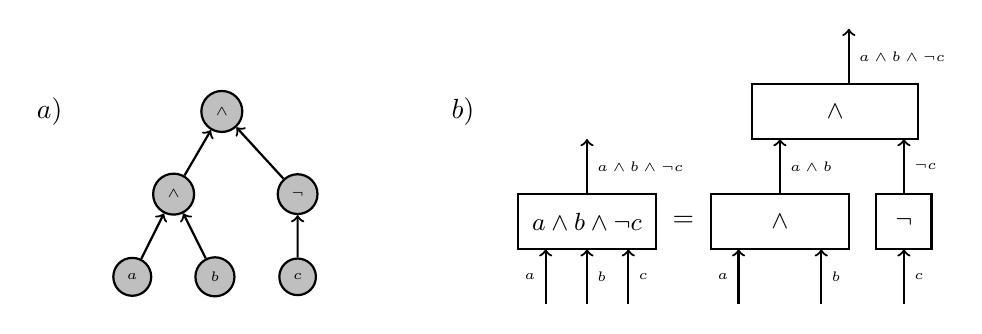
\begin{tikzpicture}[scale=0.35, yscale=-1, thick] % , baseline = -3.5pt

\begin{scope}[shift={(-15,0)}]

\node[anchor=center] (text) at (-3,-6) {${a)}$};

	\node [circle, draw, thick, fill=gray!50] (T1) at (0,0) {\tiny $\catvariableof{a}$};
	\node [circle, draw, thick, fill=gray!50] (T2) at (3,0) {\tiny $\catvariableof{b}$};
	\node [circle, draw, thick, fill=gray!50] (T3) at (6,0) {\tiny $\catvariableof{c}$};
	
	\node [circle, draw, thick, fill=gray!50] (and) at (1.5,-3) {\tiny $\land$};
	\node [circle, draw, thick, fill=gray!50] (not) at (6,-3) {\tiny $\lnot$};	
	
	\draw [->] (T1) -- (and);
	\draw [->] (T2) -- (and);
	
	\draw [->] (T3) -- (not);	
	
	\node [circle, draw, thick, fill=gray!50] (head) at (3.25,-6) {\tiny $\land$};
	
	\draw [->] (and) -- (head);
	\draw [->] (not) -- (head);			
\end{scope}

\node[anchor=center] (text) at (-3,-6) {${b)}$};

\draw[->] (0,1)--(0,-1) node[midway,left] {\tiny $\catvariableof{a}$}; 
\draw[->] (1.5,1)--(1.5,-1) node[midway,right] {\tiny $\catvariableof{b}$}; 
\draw[->] (3,1)--(3,-1) node[midway,right] {\tiny $\catvariableof{c}$}; 
\draw (-1,-1) rectangle (4, -3);
\node[anchor=center] (text) at (1.5,-2) {\small $\rencodingof{a \land b \land \lnot c}$};
\draw[->] (1.5,-3)--(1.5,-5) node[midway,right] {\tiny $\headvariableof{a \land b \land \lnot c}$}; 

\node[anchor=center] (text) at (5,-2) {${=}$};


\begin{scope}[shift={(7,0)}]

\draw[->] (0,1)--(0,-1) node[midway,left] {\tiny $\catvariableof{a}$}; 
\draw[->] (3,1)--(3,-1) node[midway,right] {\tiny $\catvariableof{b}$}; 
\draw[->] (6,1)--(6,-1) node[midway,right] {\tiny $\catvariableof{c}$}; 
	
\draw (-1,-1) rectangle (4, -3);
\node[anchor=center] (text) at (1.5,-2) {\small $\rencodingof{\land}$};

\draw[->] (1.5,-3) --(1.5,-5) node[midway,right]{\tiny $\headvariableof{a \land b}$};

\draw (5,-1) rectangle (7, -3);
\node[anchor=center] (text) at (6,-2) {\small $\rencodingof{\lnot}$};

\draw[->] (6,-3) --(6,-5) node[midway,right]{\tiny $\headvariableof{\lnot c}$};
	
\draw (0.5,-5) rectangle (6.5,-7);
\node[anchor=center] (text) at (3.5,-6) {\small $\rencodingof{\land}$};
	
\draw[->] (4,-7) -- (4,-9) node[midway,right] {\tiny $\headvariableof{a \land b \land \lnot c}$};

%\draw (3,-9) rectangle (5,-11);
%\node[anchor=center] (text) at (4,-10) {$\truevectorat{}$};

\end{scope}

\end{tikzpicture}
\end{center}
\caption{Decomposition of the formula tensor to $\exformula = a \land b \land \lnot c$ into unary (matrix) and binary (third order tensor) cores.
	a) Visualization of $\exformula$ as a graph.
	b) Tensor Network decomposition of $\exformula$.
	We can make use of the invariance of a Hadamard product with a constant tensor $\ones$ and thus not draw axis to atoms not affected by a formula.}
\label{fig:decompositionExample}
\end{figure}

\begin{remark}[Tensor Network Decomposition of Formulas]
	The decomposition of the propositional into a tensor network is a hierarchical decomposition of the formula tensor, which we will describe in more detail in \secref{sec:HT}.
	Of special interest are tree hypergraphs, where the format is called Hierarchical Tucker.
	At each decomposition of a formula into sub-formulas, two subspaces spanned by the respective atomic spaces are selected. 
\end{remark}


\subsect{Syntactical decomposition of formulas}\label{sec:termClauseDecomposition}

% Decomposition in case of missing 
We have seen how the decomposition of complex formulas into connectives acting on the component formulas can be exploited to find effective representations of the semantics by tensor networks.
Here the question arises here, how to perform such decompositions in case of a missing syntactical representation of a formula.
By \defref{def:formulas} any binary tensor is a formula.
We show in the following, how we can find a syntactic specification of a formula given its tensor.

%
%Let us now show that any formula tensor can be decomposed into a network of these connective symbols and atomic formula tensors.


\begin{definition}[Terms and Clauses]\label{def:clauses}
	Given two disjoint subsets $\nodesof{0}$ and $\nodesof{1}$ of $[\atomorder]$, the corresponding term is the formula defined on the indices $\shortcatindices\in\atomstates$ by
		\[ \termofat{\nodesof{0}}{\nodesof{1}}{\shortcatvariables}
		=\left( \bigwedge_{\atomenumerator\in\nodesof{0}} \lnot\formulaof{\atomenumerator} \right)  \land \left( \bigwedge_{\atomenumerator\in\nodesof{1}} \formulaof{\atomenumerator} \right)  \]
	and the corresponding clause is the formula defined on the indices $\catindices\in\atomstates$ by
		\[ \clauseofat{\nodesof{0}}{\nodesof{1}}{\shortcatvariables}
		=\left( \bigvee_{\atomenumerator\in\nodesof{0}} \formulaof{\atomenumerator} \right)  \lor \left( \bigvee_{\atomenumerator\in\nodesof{1}} \lnot\formulaof{\atomenumerator} \right)  \, , \]
	where by $\land_{\atomenumerator\in\nodes}$ and $\lor_{\atomenumerator\in\nodes}$ we refer to the $n$-ary connectives $\land$ and $\lor$.
	%We call the clause a minterm, if $\nodesof{0}\cup\nodesof{1} = [\atomorder]$.
	We call the term a minterm and the clause a maxterm, if $\nodesof{0}\cup\nodesof{1} = [\atomorder]$.
\end{definition}

%% 
Terms and Clauses have for any index tuple $\shortcatindices$ a polynomial representation by
		\[ \termof{\nodesof{0}}{\nodesof{1}}[\indexedshortcatvariables] 
		= \left( \prod_{\atomenumerator \in \nodesof{0}} (1-\catindexof{\atomenumerator}) \right)
		\left(  \prod_{\atomenumerator \in \nodesof{1}} \catindexof{\atomenumerator} \right) \]
and
		\[ \clauseof{\nodesof{0}}{\nodesof{1}}[\indexedshortcatvariables] 
		= 1 - \left( \prod_{\atomenumerator \in \nodesof{0}} (1-\catindexof{\atomenumerator})\right)
		\left(  \prod_{\atomenumerator \in \nodesof{1}} \catindexof{\atomenumerator} \right) \, . \]


\begin{lemma}\label{lem:termClauseOneHot}
	Terms are contractions of one-hot encodings, that is for any disjoint subsets $\nodesof{0},\nodesof{1}\subset[\atomorder]$ we have
		\[ \termof{\nodesof{0}}{\nodesof{1}}[\shortcatvariables] = \contractionof{\onehotmapof{\{\catindexof{\atomenumerator}=0 : \atomenumerator\in\nodesof{0} \} \cup \{\catindexof{\atomenumerator}=1 : \atomenumerator\in\nodesof{1}\}}}{\shortcatvariables} \, . \]
	Clauses are substractions of one-hot encodings from the trivial tensor, that is for any disjoint subsets $\nodesof{0},\nodesof{1}\subset[\atomorder]$ we have
		\[ \clauseof{\nodesof{0}}{\nodesof{1}}[\shortcatvariables] = 
		\onesat{\shortcatvariables} -
		\contractionof{\onehotmapof{\{\catindexof{\atomenumerator}=0 : \atomenumerator\in\nodesof{0} \} \cup \{\catindexof{\atomenumerator}=1 : \atomenumerator\in\nodesof{1}\}}}{\shortcatvariables} \, . \]
\end{lemma}


	
%
The reference of the formulas in the case $\nodesof{0}\dot{\cup}\nodesof{1} = [\atomorder]$ as minterms and maxterms is due to the fact, that minterms are formulas with unique models and maxterms are formulas with a unique world not satisfying the formula.
% Enumeration by $\atomstates$
We use this insight and enumerate maxterms and minterms by the index $\catindex\in\atomstates$ of the unique world where the minterm is satisfied, respectively the maxterm is not satisfied.
For any $\nodesof{0}\dot{\cup}\nodesof{1} = [\atomorder]$ we take the index tuple $\catindices$ where $\catindexof{\atomenumerator}=0$ if $\atomenumerator\in\nodesof{0}$ and $\catindexof{\atomenumerator}=1$ if $\atomenumerator\in\nodesof{1}$ and define
\begin{align*}
	\maxtermof{\catindices} = \clauseof{\nodesof{0}}{\nodesof{1}} \quad \text{and} \quad \mintermof{\catindices} = \termof{\nodesof{0}}{\nodesof{1}} \, .
\end{align*}


\begin{corollary}
	Minterms are basis elements of the tensor space, that is for any $\shortcatindices\in\atomstates$ we have
	\begin{align*}
		\mintermof{\shortcatindices} = \onehotmapofat{\shortcatindices}{\shortcatvariables}
	\end{align*}
	Maxterms are substraction of basis elements from the trivial tensor, that is for any $\shortcatindices\in\atomstates$ we have
	\begin{align*}
		\maxtermof{\shortcatindices} = \onesat{\shortcatvariables} - \onehotmapofat{\shortcatindices}{\shortcatvariables}  \, .
	\end{align*}
\end{corollary}
\begin{proof}
	Follows from \lemref{lem:termClauseOneHot}, since when $\nodesof{0}\cup\nodesof{1} = [\atomorder]$ the contraction of the one-hot encodings coincides with the one-hot encoding of a fully specified state.
\end{proof}


Based on this insight, we can decompose any propositional formula into a conjunction of maxterms or a disjunction of minterms as we show next.

\begin{theorem}\label{the:tensorToMaxMinTerms}
	For any boolean tensor $\hypercoreat{\shortcatvariables}\in\atomspace$ with leg-dimensions two we have
	\begin{align*}
		\hypercoreat{\shortcatvariables} = \left( \bigvee_{\hyperonecoordinates} 
		\termof{\catzeropositions}{\catonepositions} 
		\right)
		[\shortcatvariables] 
	\end{align*}
	and
	\begin{align*}
		\hypercoreat{\shortcatvariables} = \left( \bigwedge_{\hyperzerocoordinates} 
		\clauseof{\catzeropositions}{\catonepositions} 
		\right)
		[\shortcatvariables] \, .
	\end{align*}
\end{theorem}
\begin{proof}
	To show the representation by minterms we use the decomposition
	\begin{align*}
		\hypercoreat{\shortcatvariables}  = \sum_{\hyperonecoordinates} \onehotmapofat{\shortcatindices}{\shortcatvariables}
	\end{align*}
	and notice that each term in the disjunction modifies the formula by adding respective world $\shortcatindices$ to the models of the formula.
	To show the representation by maxterms we use the decomposition
	\begin{align*}
		\hypercoreat{\shortcatvariables}  = \onesat{\shortcatvariables} \quad - \sum_{\hyperzerocoordinates} \onehotmapofat{\shortcatindices}{\shortcatvariables}
	\end{align*}
	and notice that each term in the conjunction modifies the formula by removing the respective world $\shortcatindices$ from the models of the formula.	
	Thus, both decompositions are propositional formulas with the same set of models as the formula $\hypercore$ and are thus identical to $\hypercore$.
\end{proof}


% Canonical normal forms
The decompositions found in \theref{the:tensorToMaxMinTerms} are also called canonical normal forms to propositional formulas $\hypercoreat{\shortcatvariables}$.

%% Universality of representations
\begin{remark}[Efficient Representation in Propositional Syntax]
	% Relation with binary CP
	The decomposition in \theref{the:tensorToMaxMinTerms} is a basis CP decomposition of the binary tensor and will further be investigated in \charef{cha:sparseCalculus}.
	The formulas constructed in the proof of \theref{the:tensorToMaxMinTerms} are however just one possibility to represent a formula tensor in propositional syntax.
	Typically there are much sparser representations for many formula tensors, in the sense that less connectives and atomic symbols are required.
	Having such a sparser syntactical description of a propositional formula can be exploited to find a shorter conjunctive normal form of the formula and construct a sparse polynomial based on similar ideas as in \theref{the:tensorToMaxMinTerms}.
	%One way to eliminate syntactical redundancies are through schemes for decompositions called normal forms, for example the Conjunctive Normal Form (CNF) or the Disjunctive Normal Form (DNF).
	We will provide such constructions in \charef{cha:sparseCalculus}, where we show that dropping the demand of directionality and investigating binary CP Decompositions will improve the sparsity of the polynomial formula representation.
\end{remark}

\subsect{Comparing with probabilistic approaches }

Both probability and logic provide a human-understandable interface to machine learning.
As we will describe in \parref{par:two}, they can be combined in one formalism providing efficient reasoning.

% Same thesises repeated??
\textbf{Probability} represents the uncertainty of states.
The categorical variables are called random variables and their joint distribution is represented by a probability tensor.
Humans interpret probabilities by Bayesian and frequentist approaches.
Reasoning based on Bayes Theorem has an intuitive interpretation in terms of evidence based update of prior distributions to posterior distributions.
However it is based on interpreting (large amounts) of numbers, which makes it hard for humans to assess the probabilistic reasoning process.

\textbf{Logics} explains relations between sets of worlds in a human understandable way.
Categorical variables have dimension $2$, where the first is interpreted as indicating a $\falsesymbol$ state and the second as a $\truesymbol$ state.
We mainly restrict to propositional logics, where there are finite sets of such variables called atomic formulas.
Using model-theoretic semantics it defines entailment of sets by other sets, which is understandable as a consequence relation.

\textbf{Tensors} unify both approaches since they are natural numerical structures to represent properties of states in factored systems.
The potential is then based in employing scalable multilinear algorithms to solve reasoning problems.
Further, algorithms formulated in tensor networks have a high parallelization potential, which is why they are of central interest in the development of AI-dedicated software and hardware.

The different areas have developed separated languages to describe similar objects.
Here we want to provide a rough comparison of those in a dictionary.

\begin{tabular}{l|l|l|l}
    & \textbf{Probability Theory} & \textbf{Propositional Logic} & \textbf{Tensors}   \\
    \hline
    \textit{Atomic System}        & Random Variable             & Atomic Formula               & Vector             \\
    \textit{Factored System}      & Joint Distribution          & Knowledge Base               & Tensor             \\
    \textit{Categorical Variable} & Random Variable             & Atomic Formula               & Axis of the Tensor
\end{tabular}

While the probability theory lacks to provide an intuition about sets of events, propositional syntax has limited functionality to represent uncertainties.
Tensors on the other side can build a bridge by representing both functionalities and relying on probability theory and logics for respective interpretations.


\sect{Outlook}

While we in this chapter investigated representation schemes for single propositional formulas, we will further study the representation of knowledge bases consisting in multiple formulas in \secref{sec:hardNetworks}.
Further, we will build hybrid models bridging the concepts of probability distributions and propositional logics in \secref{sec:hybridNetworks}.
Propositional formulas will therein serve as features and base measures for exponential families.
%Further study of representing Knowledge Bases based on Tensor Networks of its formulas in \secref{sec:hardNetworks} (see \theref{the:conDecKB}).